% Standalone preview of the Section 5.2 draft, the Chapter 6 paragraphs, and Appendix A.
% Compile from this folder: pdflatex preview.tex (twice). The figures are copied into ./figures/ by
% Section 12 of result_5_2.ipynb (from result_5_2/); the tex files are read from the parent folder.
% Same class options as main.tex; the relevant parts of settings.tex; pdfLaTeX + mathpazo (Palatino).
\documentclass[headsepline,footsepline,footinclude=false,oneside,fontsize=11pt,paper=a4,listof=totoc,bibliography=totoc,DIV=12]{scrbook}
\PassOptionsToPackage{table,svgnames,dvipsnames}{xcolor}
\usepackage[utf8]{inputenc}
\usepackage[T1]{fontenc}
\usepackage[sc]{mathpazo}
\usepackage[english]{babel}
\usepackage[autostyle]{csquotes}
\usepackage{scrlayer-scrpage}
\automark[section]{section}
\ihead{}\chead{\headmark}\ohead{}
\usepackage{xcolor}
\usepackage{amsmath}
\usepackage{amssymb}
\usepackage{tabularx}
\usepackage{graphicx}
\usepackage{booktabs}
\usepackage[final]{microtype}
\usepackage{caption}
\usepackage{multirow}
\usepackage{array}
\usepackage{makecell}
\usepackage{threeparttable}
\usepackage{url}
\usepackage[hidelinks]{hyperref}
\setkomafont{disposition}{\normalfont\bfseries}
\linespread{1.05}
\RedeclareSectionCommand[
  runin=false,
  afterindent=false,
  beforeskip=1.0\baselineskip plus .2\baselineskip minus .2\baselineskip,
  afterskip=.5\baselineskip plus .1\baselineskip minus .1\baselineskip
]{paragraph}
\graphicspath{{figures/}}
\makeatletter
% Cross-references into other chapters, resolved to the numbers of main.pdf (2026-09-21, 18:25).
\newlabel{subsec:error_conditioned_preference_scoring}{{4.4.2}{29}{}{subsection.4.4.2}{}}
\newlabel{subsec:preference_pair_construction}{{4.4.3}{34}{}{subsection.4.4.3}{}}
\newlabel{tab:first_turn_error_move_cooccurrence}{{4.5}{31}{}{table.4.5}{}}
\newlabel{tab:first_turn_error_move_ppmi}{{4.6}{33}{}{table.4.6}{}}
\newlabel{subsec:preprocessing_data_and_input_rep}{{4.3.1}{15}{}{subsection.4.3.1}{}}
\newlabel{chapter:Discussions}{{6}{58}{}{chapter.6}{}}
\newlabel{subsec:candidate_tutor_response_generation}{{4.4.1}{28}{}{subsection.4.4.1}{}}
\newlabel{subsec:selected_classifier}{{5.1.2}{53}{}{subsection.5.1.2}{}}
\newlabel{sec:pedagogical_alignment_and_evaluation_of_LLM_tutors}{{4.5}{35}{}{section.4.5}{}}
\newlabel{tab:dpo_split}{{4.8}{43}{}{table.4.8}{}}
\makeatother

\begin{document}
\selectlanguage{english}

\pagenumbering{arabic}
\setcounter{page}{55}
\setcounter{chapter}{5}
\setcounter{section}{1}
\setcounter{figure}{6}
\setcounter{table}{1}

\noindent\textbf{Preview of the Section 5.2 draft} \hfill \small compiled \today\ from \texttt{result\_5\_2/text/}\normalsize

\medskip
\noindent\small Standalone compile with the thesis class and fonts. Cross-references to Chapters 4--6 are resolved to the numbers of the current \texttt{main.pdf}; figure and table numbers continue from the current Chapter 5 (Figure 5.6, Table 5.1), so they will shift once the text is merged. Figures are the PDFs in \texttt{result\_5\_2/}. The Chapter 6 paragraphs and the two appendix sections (one context per error type, Figure A.1; the posterior comparison over all pairs, Figure A.2 and Table A.1) follow after the section.\normalsize

\bigskip
% =========================================================
% 5.2  Error-Conditioned Pedagogical Signals in the Constructed Preference Dataset
% ---------------------------------------------------------
% Draft for chapters/05_results.tex (Research Question 1). Replaces the section skeleton.
% Figures: result_5_2/fig_5_6_associations, fig_5_7_context_ranking, fig_5_8_posterior_shift,
%          fig_5_11_margin_by_pair, fig_5_12_model_composition, and the appendix figure fig_A_contexts (appendix_A_contexts.tex);
%          all built by result_5_2.ipynb at the repository root, to be copied into
%          __Thesis_writing/TUM_Template/figures/ by hand.
% Every number below is read off one of the figures, the table, or the appendix figure.
% Section 4.5.3 (DPO subsets) is not referenced; the margin paragraph describes the pairs only.
% =========================================================
\section{Error-Conditioned Pedagogical Signals in the Constructed Preference Dataset}\label{sec:preference_signal_results}
This section addresses Research Question~1. Section~\ref{subsec:observed_associations} reports the associations between student error types and first-turn tutor moves that the scoring method of Section~\ref{subsec:error_conditioned_preference_scoring} builds on. Section~\ref{subsec:associations_in_pairs} then examines whether these associations are reflected in the 24,298 preference pairs that Section~\ref{subsec:preference_pair_construction} constructs from the 48,839 candidate responses of the 693 training contexts. All figures are computed from the saved candidate table and the saved preference pairs; no response was generated or re-scored for this section.

% ---------------------------------------------------------
\subsection{Observed Error--Pedagogy Associations in the Source Dataset}\label{subsec:observed_associations}
Figure~\ref{fig:associations} shows the first-turn co-occurrence table of Table~\ref{tab:first_turn_error_move_cooccurrence} in two views: on the left, the observed counts, that is, the number of training contexts whose first tutor turn carries each move, per error type; on the right, the PPMI utilities of Table~\ref{tab:first_turn_error_move_ppmi} that the scoring method derives from these counts.

    \begin{figure}[!t]
        \centering
        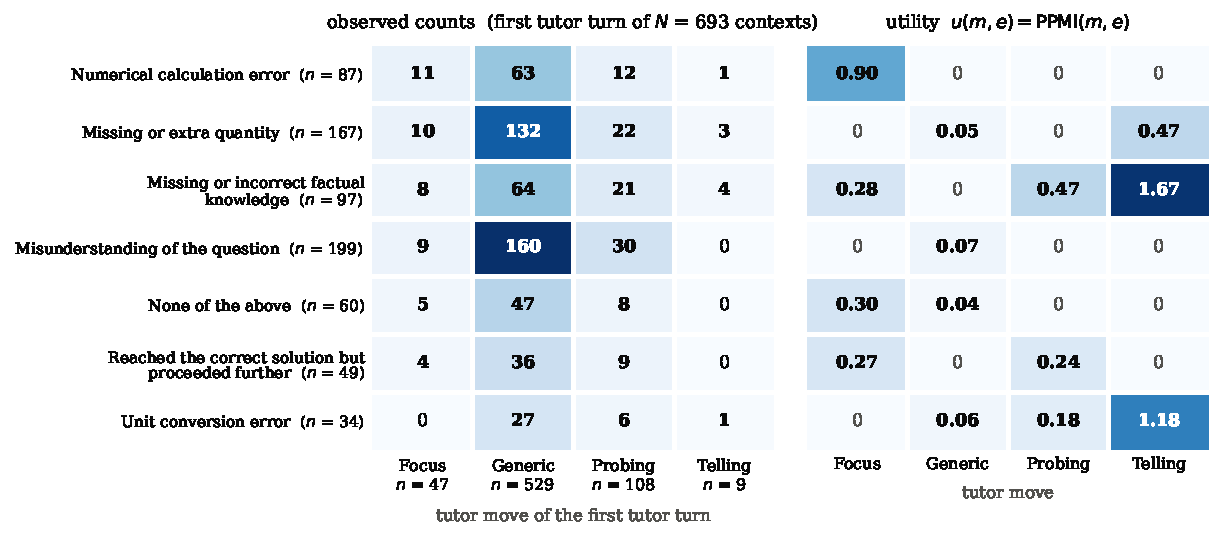
\includegraphics[width=\textwidth]{figures/fig_5_6_associations.pdf}
        \caption{Observed associations between student error types and first-turn tutor moves in 693 dialogue contexts from the training split of the aligned dataset. Left: number of contexts whose first tutor turn carries each move, per error type (the counts of Table~\ref{tab:first_turn_error_move_cooccurrence}), with the number of contexts per error type in brackets and the number of first turns per move below each move name. Right: the corresponding utility \(u(m,e)=\operatorname{PPMI}(m,e)\) of Table~\ref{tab:first_turn_error_move_ppmi}. In both panels, darker cells hold larger values.}
        \label{fig:associations}
    \end{figure}

    \paragraph{Co-occurrence and PPMI Patterns}
    \textit{Generic} is the most frequent first move for every error type: it accounts for 529 of the 693 first tutor turns, from 27 of the 34 turns of \textit{unit conversion error} to 160 of the 199 turns of \textit{misunderstanding of the question}. \textit{Probing} follows with 108 first turns, \textit{Focus} with 47, and \textit{Telling} with 9. The right panel shows how PPMI turns this frequency picture into a different one. Of the 28 cells, 14 have a positive utility and 14 are zero, and every error type has between one and three moves with a positive utility: one for \textit{numerical calculation error} (\textit{Focus}) and for \textit{misunderstanding of the question} (\textit{Generic}), two for \textit{missing or extra quantity}, \textit{none of the above}, and \textit{reached the correct solution but proceeded further}, and three for \textit{missing or incorrect factual knowledge} and \textit{unit conversion error}. Because the score \(s(r,e)\) is the posterior-weighted sum of these utilities, the zero cells define what the scoring does not reward: posterior mass on a zero-utility move adds nothing to the score, and, since the posterior sums to one, it is mass that the moves with a positive utility do not receive. \textit{Generic} receives a positive utility only for the four error types in which it occurs more often than its overall rate of 529 in 693 (\textit{missing or extra quantity}, \textit{misunderstanding of the question}, \textit{none of the above}, and \textit{unit conversion error}), and these are the smallest utilities in the table (0.04--0.07). The move with the largest utility differs between error types: \textit{Focus} for \textit{numerical calculation error} (0.90), \textit{none of the above} (0.30), and \textit{reached the correct solution but proceeded further} (0.27); \textit{Telling} for \textit{missing or extra quantity} (0.47), \textit{missing or incorrect factual knowledge} (1.67), and \textit{unit conversion error} (1.18); and \textit{Generic} for \textit{misunderstanding of the question} (0.07). \textit{Probing} has a positive utility for three error types (0.18--0.47) but is never the largest.

    \paragraph{Strength and Support of the Associations}
    The left panel also shows the observations behind each utility. The three largest utilities, all for \textit{Telling}, rest on three, four, and one first tutor turns out of 167, 97, and 34 contexts, respectively. The utility of \textit{Focus} for \textit{numerical calculation error} (0.90) rests on 11 of 87 contexts, and the three positive \textit{Probing} utilities on 21, 9, and 6 first turns. The utilities are therefore ordered differently from the counts: the largest values in the right panel come from the rarest move in the left panel. This property of the utilities is taken up again in Chapter~\ref{chapter:Discussions}.

% ---------------------------------------------------------
\subsection{Examining Error--Pedagogy Associations in Chosen Responses}\label{subsec:associations_in_pairs}
The scoring of Section~\ref{subsec:error_conditioned_preference_scoring} gives every candidate of a context a score, and the pairing rule of Section~\ref{subsec:preference_pair_construction} splits the ranked candidates of the context into a chosen half and a rejected half. This subsection follows the construction at four levels: two contexts in detail (Figure~\ref{fig:context_ranking} and Table~\ref{tab:example_pairs}), one context for each of the seven error types (Figure~\ref{fig:app_contexts} in Appendix~\ref{app:contexts}), the mean posterior of the chosen and of the rejected responses over all 24,298 pairs (Figure~\ref{fig:posterior_shift} in Appendix~\ref{app:posterior_comparison}), and the score margins of all pairs (Figure~\ref{fig:margin_by_pair}). In each of them, the zero cells of Figure~\ref{fig:associations} are as visible as the positive ones.

    \paragraph{Scoring of a Preference Pair}
    Figure~\ref{fig:context_ranking} follows two contexts through the scoring and pairing of Sections~\ref{subsec:error_conditioned_preference_scoring} and~\ref{subsec:preference_pair_construction}: one with a \textit{numerical calculation error} (context 609, 69 candidates, positive utility only for \textit{Focus}) and one with \textit{missing or incorrect factual knowledge} (context 150, 72 candidates, utilities of 0.28, 0.47, and 1.67 for \textit{Focus}, \textit{Probing}, and \textit{Telling}). The lower panels show the posterior of every candidate, the upper panels the resulting score, the ranking, and the first three pairs. For the \textit{numerical calculation error}, the three other utilities are zero, so the score is 0.90 times the \textit{Focus} posterior and every unit of posterior mass on \textit{Probing} or \textit{Telling} lowers it: the 34 chosen candidates all have a \textit{Focus} posterior above 0.87 and scores between 0.79 and 0.84, the score falls below 0.7 only from rank 50 onwards, and the last ten ranks are the ten candidates whose posterior is dominated by \textit{Telling} (0.50--0.70), with scores of 0.21--0.40. For \textit{missing or incorrect factual knowledge} the order is reversed, because \textit{Telling} now carries the largest utility and only \textit{Generic} is zero. The twelve candidates with a dominant \textit{Telling} posterior (0.77--0.88) occupy the first twelve ranks with scores of 1.35--1.50, the candidates that mix \textit{Focus} with some \textit{Telling} mass follow, and the 36 rejected candidates are \textit{Focus} responses with a \textit{Focus} posterior of 0.76--0.93 and scores of 0.31--0.37.

    Table~\ref{tab:example_pairs} lists the second pair (\(j=2\)) of both contexts. In both pairs, one response asks the student which quantity to recompute and the other gives the complete calculation. The scoring puts the question on the chosen side and the complete calculation on the rejected side for the \textit{numerical calculation error} (scores 0.83 against 0.24), and the complete calculation on the chosen side and the question on the rejected side for \textit{missing or incorrect factual knowledge} (1.48 against 0.31). The same two kinds of response thus receive opposite preferences under the two error types, which is the intended behavior of the utility \(u(m,e)\).

    \begin{figure}[!t]
        \centering
        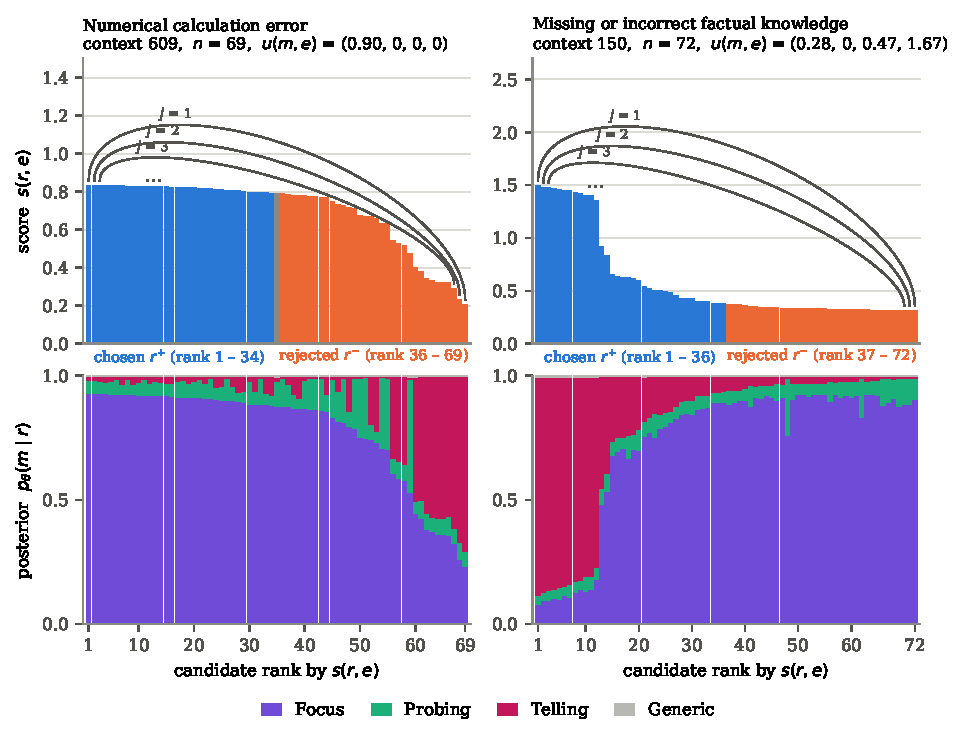
\includegraphics[width=\textwidth]{figures/fig_5_7_context_ranking.pdf}
        \caption{All candidates of two training contexts, ranked by the error-conditioned score \(s(r,e)\). Left: \textit{numerical calculation error} (context 609, \(n=69\)); right: \textit{missing or incorrect factual knowledge} (context 150, \(n=72\)). The utility vector under each title lists \(u(m,e)\) in the order \textit{Focus}, \textit{Generic}, \textit{Probing}, \textit{Telling}. Top: the score of every candidate; the blue half is chosen, the orange half rejected, and the grey middle candidate is omitted when \(n\) is odd. The arcs mark the first three pairs, which join rank \(j\) with rank \(n-j+1\). Bottom: the classifier posterior \(p_{\theta}(m\mid r)\) of the same candidates, stacked per move.}
        \label{fig:context_ranking}
    \end{figure}

    % --- Table: generated by result_5_2.ipynb -> result_5_2/text/table_example_pairs.tex ---
    \begin{table}[!t]
        \centering
        \footnotesize
        \setlength{\tabcolsep}{3pt}
        \renewcommand{\arraystretch}{1.15}
        \captionsetup{skip=4pt}
        \begin{tabularx}{\linewidth}{@{}l>{\raggedright\arraybackslash}Xlr@{}}
            \toprule
            Side & Tutor response (generation model) & \mbox{$p_{\theta}(m \mid r)$} & \mbox{$s(r, e)$} \\
            \midrule
            \multicolumn{4}{@{}l}{\textit{Numerical calculation error} (context 609), $u(m, e)$ = (0.90, 0, 0, 0)} \\
            Chosen & let's look closely at the bridge trolls: the problem says "6 less than four times that number," which means we need to multiply first before subtracting 6. can you try calculating the bridge trolls again using that rule? (gemini-3.5-flash-lite) & \mbox{(0.93, 0.00, 0.05, 0.02)} & 0.83 \\
            Rejected & “6 less than four times 6” means \(4 \times 6 - 6 = 18\) trolls under the bridge, not \(4 \times 6 + 6\). half of 18 is 9, so the total is \(6 + 18 + 9 = 33\) trolls. (gpt-5.6-terra) & \mbox{(0.26, 0.00, 0.07, 0.67)} & 0.24 \\
            \midrule
            \multicolumn{4}{@{}l}{\textit{Missing or incorrect factual knowledge} (context 150), $u(m, e)$ = (0.28, 0, 0.47, 1.67)} \\
            Chosen & the half-off offer must be used on the cheaper original pair, so the \$40 shoes cost \$20 and the \$60 shoes stay \$60, for a subtotal of \$80. a fourth of \$80 is \$20, so james pays \$80 - \$20 = \textbf{\$60}. (gpt-5.6-terra) & \mbox{(0.09, 0.01, 0.03, 0.86)} & 1.48 \\
            Rejected & you correctly found the prices of both pairs of shoes, but let's re-read carefully which pair is supposed to be "half off." which of the two prices, \$40 or \$60, is the cheaper one that gets the discount? (gemini-3.5-flash-lite) & \mbox{(0.88, 0.00, 0.11, 0.01)} & 0.31 \\
            \bottomrule
        \end{tabularx}
        \caption{Second preference pair ($j = 2$) of the two dialogue contexts in Figure~\ref{fig:context_ranking}. The dialogue context (student error type) and the corresponding utility $u(m, e)$ are shown above each pair. Posterior and utility values are listed in the order \textit{Focus}, \textit{Generic}, \textit{Probing}, \textit{Telling}; the score is their inner product.}
        \label{tab:example_pairs}
    \end{table}

    \paragraph{The Same Pattern in Every Error Type}
    Figure~\ref{fig:app_contexts} in Appendix~\ref{app:contexts} repeats Figure~\ref{fig:context_ranking} for every error type, drawing the context whose first pair has the widest normalized margin of its error type, with one row of blocks per family of the utility table. The pattern of Figure~\ref{fig:context_ranking} recurs in all seven contexts, and it follows the utility table. In the three \textit{Focus}-associated error types (first row of Figure~\ref{fig:app_contexts}), every candidate whose top label is \textit{Telling} or \textit{Probing} lies in the rejected half, at the very bottom of the ranking: 5 \textit{Telling} and 1 \textit{Probing} candidates for \textit{numerical calculation error}, 15 \textit{Probing} candidates for \textit{none of the above}, and 3 \textit{Telling} and 1 \textit{Probing} candidates for \textit{reached the correct solution but proceeded further}; the chosen halves of these three contexts consist of \textit{Focus} responses only, ordered by their \textit{Focus} posterior. In the three \textit{Telling}-associated error types (second row) the order is reversed: every candidate whose top label is \textit{Telling} stands at the top of the ranking and belongs to the chosen half (1, 12, and 11 candidates, with scores of 0.41, 1.35--1.50, and 0.57--1.05), and the rejected halves consist of \textit{Focus} responses whose scores differ only in the third decimal. For \textit{misunderstanding of the question} (third row), the only positive utility is that of \textit{Generic}, and the scores of the context stay below 0.07 with a nearly flat ranking after the first rank.

    \paragraph{Chosen--Rejected Probability Comparison}
    Figure~\ref{fig:posterior_shift} in Appendix~\ref{app:posterior_comparison} extends the comparison from the two contexts to all 24,298 pairs. For each error type and each move, it compares the mean classifier posterior of the chosen responses with that of the rejected responses. In all six error types with a \textit{Focus} or \textit{Telling} utility, the differences follow the utility table: the move with the largest utility is higher on the chosen side, and no move with zero utility is. For the three \textit{Focus}-associated error types, the mean \textit{Focus} posterior is 0.88--0.90 on the chosen side against 0.68--0.76 on the rejected side. For the three \textit{Telling}-associated error types, \textit{Telling} is higher on the chosen side (0.11--0.13 against 0.02), but the largest utility is not reflected in the largest posterior mass: \textit{Focus} remains the most probable move of the chosen responses (0.69--0.78). The utility table is thus reflected in the difference between the two sides, not in the dominant move of the chosen responses. \textit{Misunderstanding of the question} is the exception: its only positive utility belongs to \textit{Generic}, which the candidates almost never realize, so the two sides differ only marginally (0.004 against 0.002) and the scoring has nothing to prefer.

    Two properties of the data limit the \textit{Telling} side. First, the candidate pool is nearly the same for every error type and dominated by \textit{Focus}, the top label of 45,104 of the 48,839 candidates; \textit{Telling} is the top label of 1,498, and 307 of the 693 contexts hold no \textit{Telling}-labelled candidate at all (Table~\ref{tab:candidate_pool} in Appendix~\ref{app:posterior_comparison}). Second, the moves of the candidates are those assigned by the classifier of Section~\ref{subsec:selected_classifier}, which recovers about half of the \textit{Telling} utterances of its test set (F1 of 0.40), and the \textit{Telling} utilities themselves rest on one to four first tutor turns (Figure~\ref{fig:associations}). Both points are discussed in Chapter~\ref{chapter:Discussions}.

    \paragraph{Score Margins of the Constructed Pairs}
    Figure~\ref{fig:margin_by_pair} shows the score margins that the pairing rule of Section~\ref{subsec:preference_pair_construction} produces. Because pair \(j\) joins rank \(j\) with rank \(n-j+1\), the margin decreases with \(j\) in every context. The figure reports the mean normalized margin \(\Delta_{e,j}/\max_{m}\operatorname{PPMI}(m,e)\) over all contexts of each error type for the first 30 pairs of a context, the number of pairs that every context has. For the first pair, the mean lies between 0.37 (\textit{missing or incorrect factual knowledge}) and 0.71 (\textit{numerical calculation error} and \textit{none of the above}) in six of the seven error types; it is 0.03 for \textit{misunderstanding of the question}, where the three other utilities are zero and the scores of all candidates are bounded by the \textit{Generic} utility of 0.07 (third row of Figure~\ref{fig:app_contexts}). By the tenth pair the mean has fallen to 0.11--0.28, and by the thirtieth pair to 0.04 or less in every error type. The two error types with the largest \textit{Focus} utilities (\textit{numerical calculation error}, 0.90; \textit{none of the above}, 0.30) keep the widest margins at every \(j\); the other four error types with a \textit{Focus} or \textit{Telling} utility lie between 0.37 and 0.49 at the first pair and between 0.11 and 0.17 at the tenth.

    \begin{figure}[!t]
        \centering
        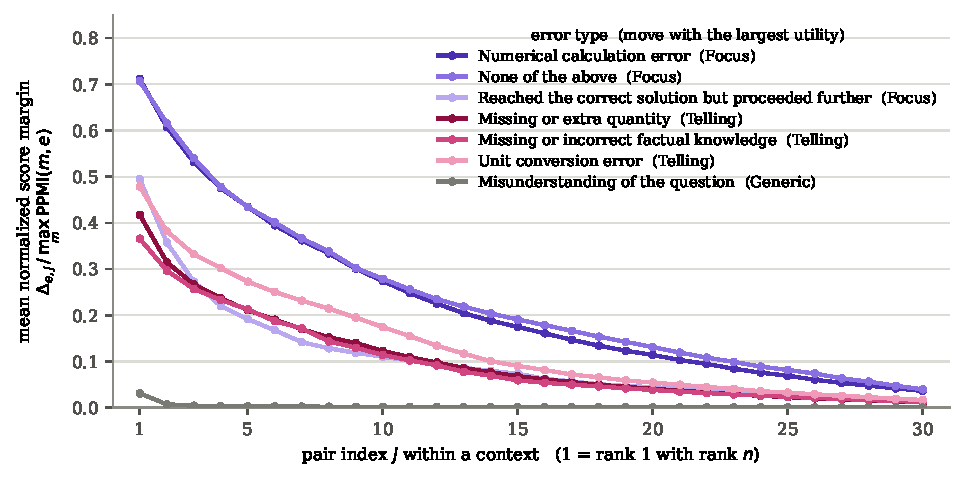
\includegraphics[width=\textwidth]{figures/fig_5_11_margin_by_pair.pdf}
        \caption[Score margins of the constructed pairs by pair index.]{Score margin of the constructed pairs by pair index \(j\) within a context (pair \(j\) joins rank \(j\) with rank \(n-j+1\)). Each point is the mean normalized margin \(\Delta_{e,j}/\max_{m}\operatorname{PPMI}(m,e)\) over all contexts of the error type. Only the first 30 pairs of every context are shown, so that every point rests on all contexts of its error type (87, 60, 49, 167, 97, 34, and 199 contexts in the order of the legend).}
        \label{fig:margin_by_pair}
    \end{figure}

    \paragraph{Generation Model of the Chosen and Rejected Responses}
    The six generation models contribute nearly equal shares of the candidate pool (15.7--17.0\,\% each) and, over all 24,298 pairs, nearly equal shares of the chosen side (12.1--19.5\,\%). Within an error type, however, the two sides differ in their model composition, and they differ in opposite directions in the two families (Figure~\ref{fig:model_composition}). For the three \textit{Telling}-associated error types, \path{gpt-5.6-terra} generates 27\,\% of the chosen but 5\,\% of the rejected responses, and \path{gemini-3.5-flash-lite} 6\,\% of the chosen but 26\,\% of the rejected responses; for the three \textit{Focus}-associated error types the picture is reversed, with \path{gpt-5.6-terra} at 5\,\% of the chosen and 26\,\% of the rejected responses. For \textit{misunderstanding of the question}, the shares of every model stay within 13--22\,\% on both sides. The pattern follows the moves that the models realize: \textit{Telling} is the top label of 12.5\,\% of the responses of \path{gpt-5.6-terra} but of at most 4\,\% of the responses of the other five models, so its responses rise to the chosen side wherever \textit{Telling} has a positive utility and fall to the rejected side wherever it has none. What this entails for preference optimization is discussed in Chapter~\ref{chapter:Discussions}.

    \begin{figure}[!t]
        \centering
        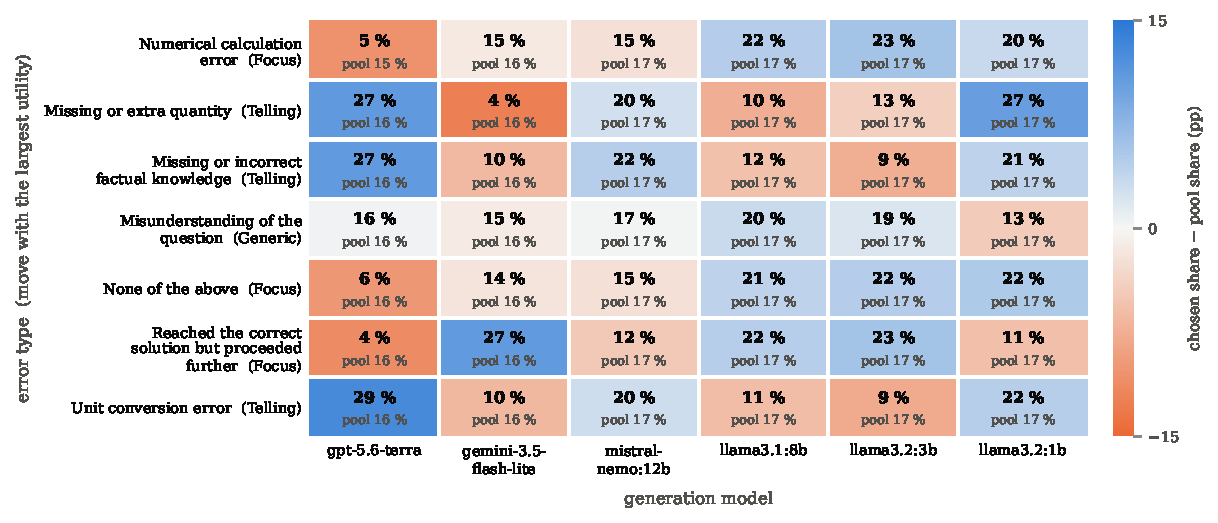
\includegraphics[width=\textwidth]{figures/fig_5_12_model_composition.pdf}
        \caption{Generation model of the chosen responses per error type. Each cell gives the share of the chosen responses of an error type that were generated by the model, with the model's share of all candidates of that error type (\textit{pool}) below; the colour shows the difference between the two in percentage points. Rows are labelled with the move that has the largest utility for the error type.}
        \label{fig:model_composition}
    \end{figure}

    \paragraph{The Preference Signal in the Constructed Dataset}
    Taken together, the figures answer the second part of Research Question~1. First, in each of the eight contexts shown (Figures~\ref{fig:context_ranking} and~\ref{fig:app_contexts}), the candidates that realize the move associated with the error type stand at the top of the ranking and become chosen, whereas the candidates that realize a move with zero utility stand at the bottom and become rejected. Second, the direction of this preference reverses between the \textit{Focus}-associated and the \textit{Telling}-associated error types: the same kind of response, a complete calculation, is rejected for \textit{numerical calculation error} and chosen for \textit{missing or incorrect factual knowledge} (Table~\ref{tab:example_pairs}). Third, the same holds on average over all 24,298 pairs: in every error type the chosen responses carry more posterior mass on the move with the largest utility than the rejected responses, and in the six error types with a \textit{Focus} or \textit{Telling} utility no move with zero utility carries more mass on the chosen side (Figure~\ref{fig:posterior_shift}). Fourth, the separation between the two halves is measurable: over all 24,298 pairs, the first pair of a context has a mean normalized margin between 0.37 and 0.71 in the six error types with a \textit{Focus} or \textit{Telling} utility (Figure~\ref{fig:margin_by_pair}). The constructed dataset therefore carries an error-conditioned preference signal for these six error types. For \textit{misunderstanding of the question}, whose only positive utility is that of \textit{Generic}, the scores are bounded by 0.07 and the margins stay close to zero (Figure~\ref{fig:margin_by_pair} and the third row of Figure~\ref{fig:app_contexts}); this case, and the fact that the signal is a difference in posterior mass while \textit{Focus} remains the most probable move of most responses on both sides (Table~\ref{tab:candidate_pool}), are taken up in Chapter~\ref{chapter:Discussions}.


\clearpage
\setcounter{chapter}{6}
\setcounter{section}{1}
\setcounter{figure}{0}
\setcounter{table}{0}
\section{Limitations and Future Work --- draft paragraphs}
\noindent\small Negative and qualifying findings about the scoring method (4.4.2) and the preference pairs (4.4.3), kept out of Section 5.2. Paragraph headings are suggestions.\normalsize

% =========================================================
% Material for Chapter 6 (Limitations and Future Work) — negative and qualifying findings
% about the error-conditioned scoring method (4.4.2) and the preference pairs (4.4.3).
% Kept out of Section 5.2 on purpose. Numbers: result_5_2.ipynb, Sections 4-6 and 8-9, and
% Final__Preference_data_Statstic_Summary__train_only.ipynb (Monte-Carlo chi-square).
% Figure fig:model_composition (result_5_2/fig_5_12_model_composition.pdf) and Table tab:candidate_pool (text/table_candidate_pool.tex)
% are placed in Section 5.2. Paragraph headings are suggestions.
% =========================================================

    \paragraph{Statistical Strength of the Error--Move Association}
    The utilities of Section~\ref{subsec:error_conditioned_preference_scoring} describe tendencies in the 693 training dialogues rather than an established association. A chi-square test of independence on the contingency table of Table~\ref{tab:first_turn_error_move_cooccurrence} gives \(\chi^{2} = 25.94\) with 18 degrees of freedom (asymptotic \(p = 0.101\)); because 10 of the 28 expected counts are below 5 and three are below 1, the \(p\)-value was also estimated with a Monte-Carlo procedure that keeps both margins fixed (200,000 resamples), which gives \(p = 0.100\). The effect size is small, with a Cram\'{e}r's \(V\) of 0.112. The null hypothesis of independence between student error type and first tutor move can therefore not be rejected at the 5\,\% level, and the direction of the association is what the PPMI table encodes, not its statistical reliability.

    \paragraph{Support Behind the Largest Utilities}
    As Figure~\ref{fig:associations} shows, the three largest utilities of the table, all for \textit{Telling} (0.47, 1.67, and 1.18), rest on three, four, and one first tutor turns. A single additional or missing \textit{Telling} turn would change these values substantially, which is the known sensitivity of PMI to rare events noted in Section~\ref{subsec:error_conditioned_preference_scoring}. The same three error types are the ones for which the scoring prefers complete-solution responses over rechecking prompts (Table~\ref{tab:example_pairs}), so the least supported utilities are also the ones with the largest effect on which responses are chosen.

    \paragraph{An Error Type Without a Usable Signal}
    For \textit{misunderstanding of the question}, the largest error type with 6,966 pairs (28.7\,\% of the dataset), the only positive utility is that of \textit{Generic} (0.075). Generated candidates almost never realize this move: \textit{Generic} is the top label of 0.04\,\% of the candidates of this error type, and their mean \textit{Generic} posterior is 0.003. The scores of all its candidates lie between 0.0001 and 0.068, the median raw score margin of its pairs is 0.0001, and 98.6\,\% of its pairs have a raw margin below 0.001 (Figure~\ref{fig:margin_by_pair}). The three pairs of the dataset whose two responses have exactly the same score also belong to this error type, and 559 candidates in total share their score with another candidate of the same context, so that their side in a pair depends on the sort order rather than on the score. The chosen and rejected labels of this error type therefore carry almost no error-conditioned information, although its pairs form more than a quarter of the data used for preference optimization. The chosen responses of this error type also carry more \textit{Probing} and \textit{Telling} posterior mass than the rejected ones (means of 0.18 against 0.11 and 0.10 against 0.03; Figure~\ref{fig:posterior_shift}), although no utility rewards these moves; the small \textit{Generic} posterior co-varies with the posterior mass outside \textit{Focus}.

    \paragraph{A Candidate Pool Dominated by \textit{Focus}}
    The candidate pool is nearly uniform across error types and is dominated by one move: of the 48,839 candidates, 45,104 have \textit{Focus} as their top label, 2,221 \textit{Probing}, 1,498 \textit{Telling}, and 16 \textit{Generic}, and the same proportions hold within every error type (Table~\ref{tab:candidate_pool}). A context holds two \textit{Telling}-labelled candidates among about 70, and 307 of the 693 contexts hold none. Two consequences follow. First, for the three \textit{Telling}-associated error types the chosen responses are still \textit{Focus}-labelled responses in 82--93\,\% of the pairs, and 82--90\,\% of all pairs have the same top label on both sides; the preference signal of these error types is a difference in posterior mass (a mean \textit{Telling} posterior of 0.11--0.13 against 0.02) rather than a change of the realized move; in the contexts without a \textit{Telling}-labelled candidate, the scoring can only prefer the \textit{Focus} responses with the larger \textit{Telling} share. Second, for the \textit{Focus}-associated error types the chosen side consists almost entirely of \textit{Focus}-labelled responses (99.9--100\,\%) and the rejected side to 85--90\,\%, so most of these pairs separate \textit{Focus} responses by the confidence of the classifier rather than by the move. Both consequences originate outside the scoring method, in the Stage~2 prompt of Section~\ref{subsec:candidate_tutor_response_generation}, which asks for tutoring responses of at most two sentences, and in the classifier of Section~\ref{subsec:selected_classifier}, which assigns 41\,\% of the \textit{Probing} utterances of its test set to \textit{Focus}.

    \paragraph{Conditioning at the Level of Move Families}
    Re-ranking the candidates of every context with the utility column of each other error type (not shown; \path{result_5_2.ipynb}, Section~6) reveals that the seven utility columns produce only three distinct preference directions. The columns of \textit{numerical calculation error} and of \textit{none of the above} select the same responses, because both have a positive utility for \textit{Focus} only among the moves that the candidates realize, and the column of \textit{reached the correct solution but proceeded further} agrees with them on 74--78\,\%; the columns of \textit{missing or incorrect factual knowledge} and \textit{unit conversion error} agree on 99\,\%. The preference dataset therefore distinguishes \textit{Focus}-associated, \textit{Telling}-associated, and \textit{Generic}-only error types, but not the individual error types within a family. Differences between error types of the same family that a preference-optimized model may show cannot be attributed to the scoring method.

    \paragraph{Generation Model as a Confound}
    The six generation models differ in the moves they realize: \textit{Telling} is the top label of 12.5\,\% of the responses of \path{gpt-5.6-terra} but of 0--4\,\% of the responses of the other five models, and \textit{Probing} of 8.2\,\% of the responses of \path{mistral-nemo:12b}. The error-conditioned scoring consequently prefers different generation models for different error types (Figure~\ref{fig:model_composition} in Section~\ref{subsec:associations_in_pairs}). Responses of \path{gpt-5.6-terra} make up 27--29\,\% of the chosen responses of the three \textit{Telling}-associated error types but only 4--6\,\% of the chosen responses of the three \textit{Focus}-associated error types, against a pool share of 15--16\,\%; responses of \path{gemini-3.5-flash-lite} make up 4\,\% of the chosen responses for \textit{missing or extra quantity} and 27\,\% for \textit{reached the correct solution but proceeded further}, against 16\,\% of the pool. The chosen and rejected sides of a pair thus differ not only in the tutor move but also, systematically, in the generation model and its style (formatting, use of inline mathematics, length: mean response length ranges from 36 words for \path{mistral-nemo:12b} to 65 words for \path{llama3.2:1b}). A preference-optimized model can learn these stylistic differences instead of, or in addition to, the intended move.


    \paragraph{Incomparable Score Scales}
    The scores of different error types live on different scales, because each is bounded by the largest utility of its error type (0.075 for \textit{misunderstanding of the question}, 1.667 for \textit{missing or incorrect factual knowledge}). Margins were therefore normalized by that maximum before any comparison or selection across error types, but the normalization does not equalize the distributions: the mean normalized margin of the first pair ranges from 0.37 to 0.71 among the six error types with a usable signal (Figure~\ref{fig:margin_by_pair}), so the same selection ratio retains pairs of different separation in different error types.

    \paragraph{Association, Not Pedagogical Validity}
    Finally, a chosen response is one that realizes the move most associated with the error type in the training dialogues, not one that was judged pedagogically better. Table~\ref{tab:example_pairs} makes the consequence concrete: for \textit{numerical calculation error} the scoring prefers a prompt to recheck one step over the complete solution, whereas for \textit{missing or incorrect factual knowledge} it prefers the complete solution over the prompt. Whether either preference is the better tutoring decision was not evaluated, and the association it rests on is, as noted above, weak and thinly supported for the \textit{Telling} cases.


\clearpage
\setcounter{chapter}{1}
\setcounter{section}{0}
\setcounter{figure}{0}
\setcounter{table}{0}
\renewcommand{\thechapter}{A}
\renewcommand{\thefigure}{A.\arabic{figure}}
\renewcommand{\thetable}{A.\arabic{table}}
\chead{Appendix A --- Dataset}
% =========================================================
% Appendix: one context per error type in a single figure, same layout as Figure fig:context_ranking (Section 5.2.2).
% Figure: result_5_2/fig_A_contexts.pdf (built by result_5_2.ipynb, Section 7b; selection rule: widest first pair).
% Add to pages/appendix.tex (or a new chapter in the appendix) and copy the PDF into figures/.
% =========================================================
\section{One Context per Student Error Type}\label{app:contexts}
Figure~\ref{fig:app_contexts} repeats Figure~\ref{fig:context_ranking} for every student error type. For each error type, the context shown is the one whose first preference pair has the widest normalized score margin \(\Delta_{e,1}/\max_{m}\operatorname{PPMI}(m,e)\) of that error type, that is, the context in which the error-conditioned scoring separates the two sides most clearly. The blocks are arranged by the move with the largest utility of the error type: the first row holds the three \textit{Focus}-associated error types, the second row the three \textit{Telling}-associated error types, and the third row the error type whose only positive utility is that of \textit{Generic}. In every block, the upper panel shows the score \(s(r,e)\) of all candidates of the context ranked from the largest to the smallest, with the chosen half in blue, the rejected half in orange, and the omitted middle candidate in grey when the number of candidates is odd; the arcs mark the first three pairs, which join rank \(j\) with rank \(n-j+1\). The lower panel shows the classifier posterior \(p_{\theta}(m\mid r)\) of the same candidates, stacked per move. The utility vector in each title lists \(u(m,e)\) in the order \textit{Focus}, \textit{Generic}, \textit{Probing}, \textit{Telling}. Context 150 (\textit{missing or incorrect factual knowledge}) is the right-hand context of Figure~\ref{fig:context_ranking}.

    \begin{figure}[p]
        \centering
        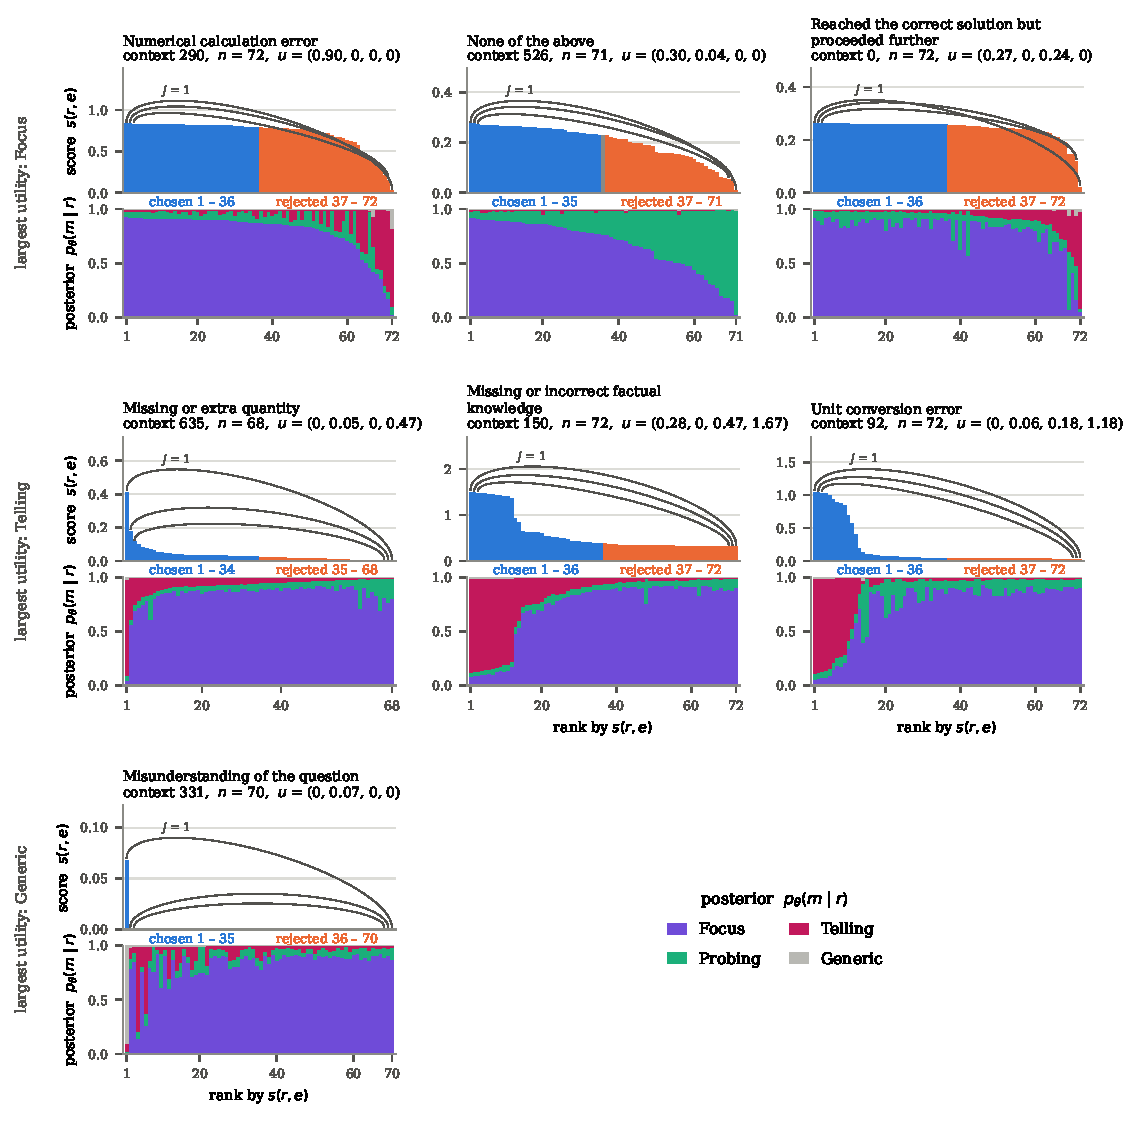
\includegraphics[width=\textwidth]{figures/fig_A_contexts.pdf}
        \caption{One context per student error type, drawn as in Figure~\ref{fig:context_ranking}: the score of all candidates of the context ranked by \(s(r,e)\) (upper panel of each block; blue: chosen half, orange: rejected half, arcs: the first three pairs) and the classifier posterior of the same candidates (lower panel). Rows group the error types by the move with the largest utility. For each error type, the context whose first pair has the widest normalized margin is shown; the block title gives the context, the number of candidates \(n\), and the utility vector \(u = (u_{\text{Focus}}, u_{\text{Generic}}, u_{\text{Probing}}, u_{\text{Telling}})\).}
        \label{fig:app_contexts}
    \end{figure}


\clearpage
% =========================================================
% Appendix: the chosen-vs-rejected posterior comparison over all pairs (Figure fig:posterior_shift) and the move
% distribution of the candidate pool (Table tab:candidate_pool), with the full description. Section 5.2.2
% ("Chosen--Rejected Probability Comparison") keeps a short summary of this appendix.
% Figure: result_5_2/fig_5_8_posterior_shift.pdf (built by result_5_2.ipynb, Section 4); table: result_5_2/text/table_candidate_pool.tex (Section 8).
% Add to pages/appendix.tex after the section of appendix_A_contexts.tex and copy the PDF into figures/.
% =========================================================
\section{Chosen and Rejected Responses over All Pairs}\label{app:posterior_comparison}
Figure~\ref{fig:posterior_shift} extends the comparison of Figure~\ref{fig:context_ranking} from two contexts to all 24,298 pairs; Section~\ref{subsec:associations_in_pairs} summarizes it. For each error type and each move, the figure shows the mean classifier posterior of the chosen responses and of the rejected responses; the move with the largest utility of the error type is set in bold. In every error type, the chosen responses place more posterior mass on that move than the rejected responses. For the three error types whose largest utility belongs to \textit{Focus}, the mean \textit{Focus} posterior is 0.90 against 0.70 (\textit{numerical calculation error}), 0.89 against 0.68 (\textit{none of the above}), and 0.88 against 0.76 (\textit{reached the correct solution but proceeded further}), while \textit{Probing} and \textit{Telling}, both with zero utility, are lower on the chosen side (for example 0.07 against 0.17 and 0.03 against 0.13 for \textit{numerical calculation error}). For the three error types whose largest utility belongs to \textit{Telling}, the pattern is the mirror image. \textit{Telling} is higher on the chosen side: 0.11 against 0.02 (\textit{missing or extra quantity}), 0.11 against 0.02 (\textit{missing or incorrect factual knowledge}), and 0.13 against 0.02 (\textit{unit conversion error}). \textit{Probing} is also higher on the chosen side where it has a positive utility (0.20 against 0.10 and 0.15 against 0.09). \textit{Focus} is lower on the chosen side (0.69 against 0.87 and 0.72 against 0.89) or equal on both sides (0.78 against 0.78 for \textit{missing or extra quantity}, where \textit{Focus} has zero utility). In all six error types with a \textit{Focus} or \textit{Telling} utility, the differences therefore follow the utility table: the move with the largest utility is higher on the chosen side, and no move with zero utility is. For these three error types, however, the largest utility is not reflected in the largest posterior mass: \textit{Focus} remains the most probable move of the chosen responses (0.69--0.78), and \textit{Telling} reaches only 0.11--0.13. The utility table is thus reflected in the difference between the chosen and the rejected side, not in the dominant move of the chosen responses. \textit{Misunderstanding of the question} is the exception. Its only positive utility belongs to \textit{Generic}, but the candidates almost never realize this move, so the two sides differ only marginally on \textit{Generic} (0.004 against 0.002) and the scoring has nothing to prefer; the differences on \textit{Probing} (0.18 against 0.11) and \textit{Telling} (0.10 against 0.03) arise without a utility of their own.

Two features of the figure are set by the candidate pool rather than by the utilities (Table~\ref{tab:candidate_pool}). The pool is nearly the same for every error type: \textit{Focus} is the top label of 45,104 of the 48,839 candidates and of 91 to 95\,\% of the candidates of every single error type. The differences between error types in Figure~\ref{fig:posterior_shift} therefore come from the utility column alone. And \textit{Telling} is the top label of only 1,498 candidates: a context holds two of them among about 70, and in 307 of the 693 contexts none at all, among them 81 of the 167 contexts of \textit{missing or extra quantity}, 49 of 97 for \textit{missing or incorrect factual knowledge}, and 15 of 34 for \textit{unit conversion error}. The chosen half of such a context therefore contains at most a few \textit{Telling} responses and is otherwise filled with \textit{Focus} responses, which bounds the chosen-side \textit{Telling} posterior at 0.11--0.13, although every \textit{Telling} candidate of a context lies in the chosen half (Figure~\ref{fig:context_ranking}).

Two further qualifications apply to the \textit{Telling} side of the figure. First, the moves of the candidates are those assigned by the classifier of Section~\ref{subsec:selected_classifier}, which recovers about half of the \textit{Telling} utterances of its test set (F1 of 0.40; 6 of 13, five of them assigned to \textit{Focus}); the \textit{Telling} values reported here are therefore the classifier's view and may understate the difference in the realized move. Second, the \textit{Telling} utilities themselves rest on one to four first tutor turns (Figure~\ref{fig:associations}), because \textit{Telling} occurs in only 9 of the 693 first turns and PPMI grows with the ratio of a co-occurrence to this base rate, whereas \textit{Generic}, with a base rate of 76\,\%, cannot exceed a utility of 0.39; the size of the utilities is thus set by the move distribution of the source data, and the preference direction of the three \textit{Telling}-associated error types is based on few observations. Both points are discussed in Chapter~\ref{chapter:Discussions}.

    \begin{figure}[!t]
        \centering
        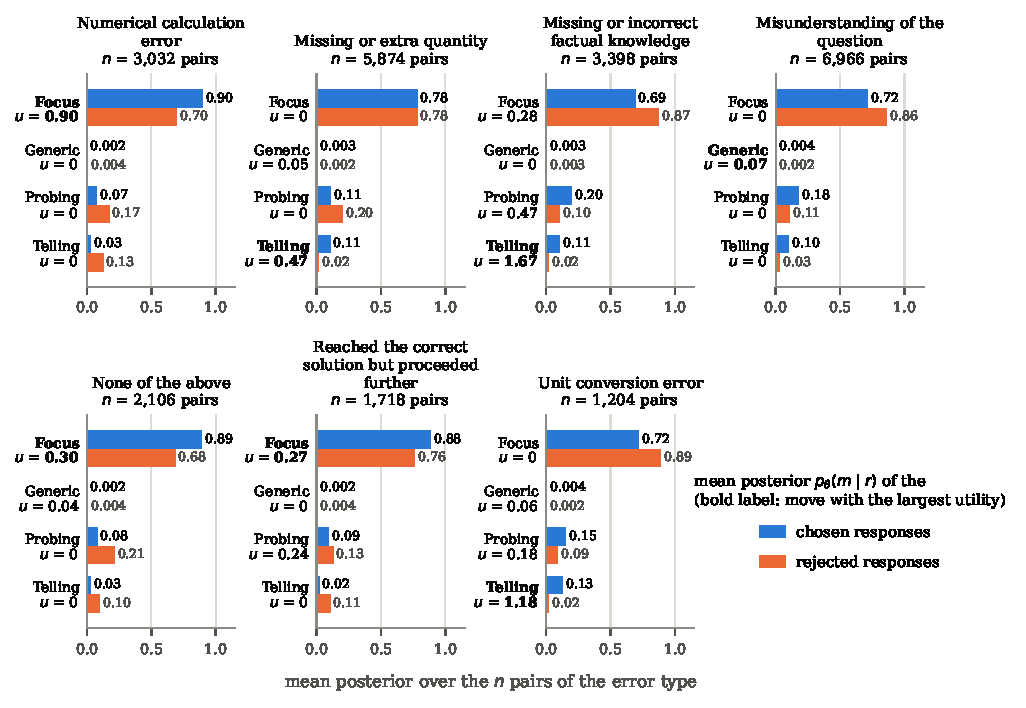
\includegraphics[width=\textwidth]{figures/fig_5_8_posterior_shift.pdf}
        \caption{Mean classifier posterior \(p_{\theta}(m\mid r)\) of the chosen responses (blue bars) and of the rejected responses (orange bars) for every move and error type, over the \(n\) pairs of the error type. The axis labels give the utility \(u(m,e)\) of the move for the error type; the move with the largest utility is set in bold.}
        \label{fig:posterior_shift}
    \end{figure}

\begin{table}[!t]
    \centering
    \footnotesize
    \setlength{\tabcolsep}{3pt}
    \renewcommand{\arraystretch}{1.08}
    \captionsetup{skip=4pt}
    \begin{tabularx}{\linewidth}{@{}>{\raggedright\arraybackslash}Xrrrrrrrrrr@{}}
        \toprule
        & & \multicolumn{4}{c}{Mean posterior $p_{\theta}(m \mid r)$} & \multicolumn{3}{c}{Top label (\%)} & \multicolumn{2}{c}{\textit{Telling} per context} \\
        \cmidrule(lr){3-6} \cmidrule(lr){7-9} \cmidrule(lr){10-11}
        Student error type & Candidates & Focus & Generic & Probing & Telling & Focus & Probing & Telling & Mean & None (\%) \\
        \midrule
        Numerical calculation error & 6,104 & 0.798 & 0.003 & 0.123 & 0.077 & 92.8 & 3.3 & 3.9 & 2.8 & 30 \\
        Missing or extra quantity & 11,808 & 0.782 & 0.003 & 0.156 & 0.060 & 92.0 & 5.3 & 2.7 & 1.9 & 49 \\
        Missing or incorrect factual knowledge & 6,826 & 0.783 & 0.003 & 0.152 & 0.063 & 91.2 & 5.6 & 3.1 & 2.2 & 51 \\
        Misunderstanding of the question & 13,997 & 0.789 & 0.003 & 0.142 & 0.066 & 92.2 & 4.6 & 3.1 & 2.2 & 45 \\
        None of the above & 4,236 & 0.788 & 0.003 & 0.147 & 0.062 & 92.5 & 4.9 & 2.6 & 1.8 & 43 \\
        Reached the correct solution but proceeded further & 3,451 & 0.823 & 0.003 & 0.112 & 0.063 & 94.9 & 2.5 & 2.6 & 1.8 & 41 \\
        Unit conversion error & 2,417 & 0.803 & 0.003 & 0.121 & 0.073 & 93.0 & 3.2 & 3.8 & 2.7 & 44 \\
        \midrule
        \textbf{All candidates} & \textbf{48,839} & \textbf{0.791} & \textbf{0.003} & \textbf{0.141} & \textbf{0.065} & \textbf{92.4} & \textbf{4.5} & \textbf{3.1} & \textbf{2.2} & \textbf{44} \\
        \bottomrule
    \end{tabularx}
    \caption{Move distribution of the candidate pool by student error type, before any ranking. For every error type: the mean classifier posterior of all its candidates for each move; the share of candidates whose top label is \textit{Focus}, \textit{Probing}, or \textit{Telling} (\textit{Generic} is the top label of at most 0.06\,\% of the candidates of any error type); and, in the last two columns, the mean number of \textit{Telling}-labelled candidates per dialogue context and the share of contexts without one. Every context holds about 70 candidates.}
    \label{tab:candidate_pool}
\end{table}


\end{document}
